\documentclass{article}%
\usepackage{amsmath}%
\usepackage{amsfonts}%
\usepackage{amssymb}%
\usepackage{graphicx}
\usepackage{amsthm}
\usepackage{wrapfig}
%-------------------------------------------
\newtheorem{theorem}{Theorem}
\newtheorem{acknowledgement}[theorem]{Acknowledgement}
\newtheorem{algorithm}[theorem]{Algorithm}
\newtheorem{axiom}[theorem]{Axiom}
\newtheorem{case}[theorem]{Case}
\newtheorem{claim}[theorem]{Claim}
\newtheorem{conclusion}[theorem]{Conclusion}
\newtheorem{condition}[theorem]{Condition}
\newtheorem{conjecture}[theorem]{Conjecture}
\newtheorem{corollary}[theorem]{Corollary}
\newtheorem{criterion}[theorem]{Criterion}
\newtheorem{definition}[theorem]{Definition}
\newtheorem{example}[theorem]{Example}
\newtheorem{exercise}[theorem]{Exercise}
\newtheorem{lemma}[theorem]{Lemma}
\newtheorem{notation}[theorem]{Notation}
\newtheorem{problem}[theorem]{Problem}
\newtheorem{proposition}[theorem]{Proposition}
\newtheorem{remark}[theorem]{Remark}
\newtheorem{solution}[theorem]{Solution}
\newtheorem{summary}[theorem]{Summary}

\theoremstyle{definition}
\newtheorem{question}{Question}

\setlength{\textwidth}{7.0in}
\setlength{\oddsidemargin}{-0.35in}
\setlength{\topmargin}{-0.5in}
\setlength{\textheight}{9.0in}
\setlength{\parindent}{0.3in}
\begin{document}

\begin{center}
    \textbf{\LARGE{Some Datastructure and Algorithm Summary} \\ \large{The time complexity of the algorithm}} \\
\end{center}

\begin{flushright}
    Kim JaeHwan
\end{flushright}

\begin{center}
    \par\noindent\line(1, 0){500}
\end{center}

\begin{section}
    {Simple Meaning of main properties of C++}


\begin{itemize}
    \item Object-oriented \\
    the benefits of OOP?
    \bigskip
    \item Generic programming
    \item Abstract data types
    \item Information hiding
    \item encapsulation
\end{itemize}

\bigskip
\end{section}

\begin{section}
    {About the time complexity}


\begin{subsection}
    {Definition and time complexity}
\end{subsection}
\noindent
Algorithm : a step-by-step procedure for solving a problem in a finite amount of time.

\bigskip\noindent
How to comopare two algorithms?

\noindent
Efficiency - Running time (time complexity), Space requirements (space complexity)

\bigskip
There are two method to check time complexity (1. Empirical studies, 2. Theoretical analysis). First method is programming and testing, but it is not exact. It can be changed by the environment such as hardware and software. So, we need to use theoretical analysis. Theoretical analysis is a high-level description of the algorithm instead of an implementation. No need to be so exact. There are three ways to compare algorithms. (1. Best case, 2. Average case, 3. Worst case)
\bigskip
\begin{enumerate}
    \item Best case(lower bound) : 
    \textbf{Big-Omega notation} \\
    $T(n)$ is $\Omega(f(n))$ if there exist a constant $c>0$ and an integer constant $n_0 \ge 1$ such that $T(n) \ge c f(n)$ for all $n \ge n_0$.
    \item Average case :
    \textbf{Big-Theta notation} \\
    $T(n)$ is $\Theta(f(n))$ if $T(n)$ is $O(f(n))$ and $\Omega(f(n))$.
    \item Worst case(upper bound) :
    \textbf{Big-Oh notation} \\
    An algorithm is $O(f(n))$ if there exist a constant $c>0$ and an integer constant $n_0 \ge 1$ such that $T(n) \le cf(n)$ for all $n \ge n_0$. Then we write $T(n) \in O(f(n))$, or $T(n) = O(f(n))$.

    This case is easier to analyze.
\end{enumerate}

\noindent
\begin{subsection}
    {Properties of Big-Oh}
\end{subsection}
Addition rule, Product Rule, and others.

There are typical growth rates:
\begin{center}
    \begin{tabular}{|rl|rl|}
        \hline
        $\Theta(1)$ & constant & $\Theta(n)$ & linear \\
        $\Theta(\log n)$ & logarithmic & $\Theta(n \log n)$ & log linear \\
        $\Theta(n^2)$ & quadratic & $\Theta(n^3)$ & cubic \\
        $\Theta(2^n)$ & exponential & $\Theta(n!)$ & factorial \\
        \hline
    \end{tabular}
\end{center}

\textbf{limitation of analysis}
\begin{itemize}
    \item Not account for constant factors, but constant factor ay dominate.
    \item Not account for different memory access times at different levels of memory hierarchy.
    \item Programs that do more computation may take less time than those that do less computation.
\end{itemize}

For example, 1000n vs $n^2$, when interested only in $n < 1000$.
For example, Cache memory $<<$ MM $<<$ HDD.

\begin{subsection}
    {Relative of Big-Oh}
\end{subsection}
\begin{enumerate}
    \item Little-oh
    \item little-omega
\end{enumerate}

\bigskip
\end{section}
\begin{section}
    {List, Stack, Queue}


\subsection*{1. List}

\subsubsection*{Definition}
A finite, \textbf{ordered} collection of elements. n. length (size) of the List

\bigskip\noindent
List Operations: Insert(x, p, L), Delete(p, L), Next(p, L), Previous(p, L), Locate(p, L), Retrieve(p, L), MakeNull(L), First(L)

\subsubsection*{Array-based list}

\begin{center}
    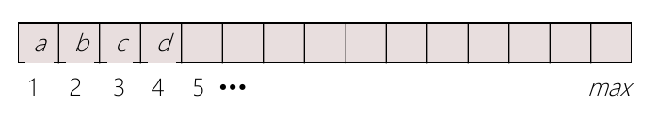
\includegraphics[]{img/arraybasedlist.png}
\end{center}
This, size n = 4
\bigskip
If execute Insert(x, 2, L), then b, c, d will be moved to the right side, then arr[index = 2] will be $x$.

\textbf{TIME COMPLEXITY} :
\begin{tabular}{ccc}
    \textbf{Insert(x, p, L)} : $O(n)$ & \textbf{Delete(p, L)} : $O(n)$ & \textbf{Locate(p, L)} : $O(1)$
\end{tabular}

\subsubsection*{Pointer-based list}

\begin{center}
    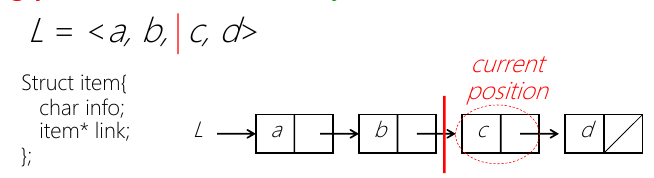
\includegraphics[]{img/pointerbasedlist.png}
\end{center}

\noindent
\textbf{- Singly-linked(one-way)} : each node has a pointer to the next node, and value.

\begin{enumerate}
    \item $P$ direcctly points to the current element.
    Difficulty for insert : hard to access to the preceding node of the current one, but we have to change the link of the preceding node. -> we need a pointer to the preceding node.
    \item \textbf{One-step ahead convention} : $P$ points to the previous element of the current position. $P$ is the position of the preceding node. \\
    When executing Insert(x, p, L) and the list is empty or the left node is empty, we can't use. Solution : add a dummy node at the beginning of the list.
\end{enumerate}

If you know the location(pointer) of the preceding node, then you can insert the new node in $O(1)$ time. But if you don't know, the time complexity is $O(n)$.

\bigskip\noindent
\textbf{- Doubly-linked(two-way)} : each node has a pointer to the next node, and the previous node, and value.
\textbf{Q}. what is the difference between singly-linked and doubly-linked?
\textbf{Solution}: In singly-linked, we can't access to the preceding node of the current one, but in doubly-linked, we can access to the preceding node of the current one. So we can get the previous node of the current one in $O(1)$ time.

The Comparison of singly-linked and doubly-linked is below.
\begin{center}
\begin{tabular}{|c|c|c|c|}
    \hline
    & \textbf{Singly-linked} & \textbf{Doubly-linked} \\
    \hline
    \textbf{Insert(x, p, L)} & $O(n)$ & $O(n)$ \\
    \hline
    \textbf{Delete(p, L)} & $O(n)$ & $O(n)$ \\
    \hline
    \textbf{Locate(p, L)} & $O(n)$ & $O(n)$ \\
    \hline
\end{tabular}
\end{center}

It is similar to the singly-linked list, but we can access to the preceding node of the current one. So we can get the previous node of the current one in $O(1)$ time.

\subsubsection*{Cursor-based list}

\begin{wrapfigure}{r}{3.1cm}
    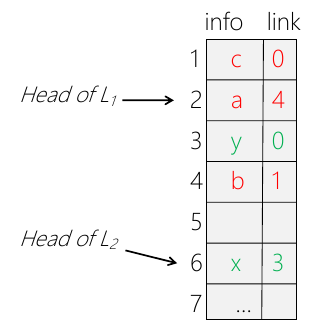
\includegraphics[width=3cm]{img/cursorbasedlist.png}
\end{wrapfigure}

\bigskip
Cursor : simulated pointer. Interger index indicating positions in array to simulate pointers. \\
\textbf{TIME COMPLEXITY} : insert(x, p, L) : $O(1)$, delete(p, L) : $O(1)$, retrieve(p, L) : $O(n)$

\bigskip

\subsection*{2. Stack}

\subsection*{Definition}

All insertion \& deletions take place at one end(Top). LIFO(Last In First Out) structure. You can implement stacks using any type of list implementation(pointer, array, cursor, ...).
\medskip
\noindent Stack Operations: Push(x, S), Pop(S), Top(S), MakeNull(S), IsEmpty(S)

\subsubsection*{Array-based Stack}
How to implement TOP? (in terms of cost of pop/push) \\
Position k(when k elements in stack): $O(1)$ \\ (Fixed) Position 1: $O(n)$

\subsubsection*{Linked stack}

\begin{wrapfigure}{c}{5.1cm}
    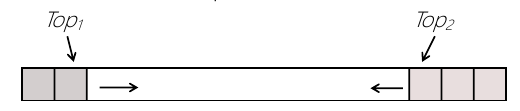
\includegraphics[width=5cm]{img/linkedstack.png}
\end{wrapfigure}

Very much similar to the pointer-based list implementation


\subsection*{3. Queue}

\subsubsection*{Definition}

FIFO(First In First Out) structure. \\
Similar to top in the stack, here we have front and rear
\medskip
\noindent Queue Operations: Enqueue(x, Q), Dequeue(Q), Front(Q), MakeNull(Q), IsEmpty(Q)

\subsubsection*{Array-based Queue}
\begin{itemize}
    \item Simple array implementation \\ "drifting queue" problem. we can solve in an inefficient way. Enqueue \& dequeue : $O(1)$ \& $O(n)$ or vice versa.

    \item \textbf{Circular Queue} 
    \begin{center}
        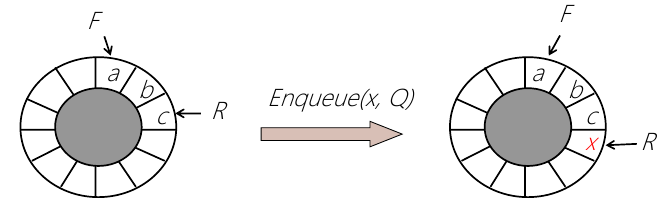
\includegraphics[scale = 0.7]{img/arraybasedqueue.png}
    \end{center}
    Modulus / Modulo operator : Methematically connect the last element to the first element via modulo operator. \\
    Then, we have a problem. How to recognize empty queue or full queue?\\
    Sol 1. Explicit count variable such as cnt. \\ Sol 2. Boolearn variable `isEmpty'
\end{itemize}

\subsubsection*{Linked Queue}
\begin{itemize}
    \item without dummy header,
    Two pointers : (F, R) Empty(Q) is true if F = R = NULL. \\ Enqueue(x, Q) also can, but Problem: Can we use the same code when inserting into an empty queue?
    \item with dummy header,
    Empty(Q) is true if F = R = header.
\end{itemize}

Comparison with header and without header.
Speed? Space utilization? Code conciseness? - insertion into an empty queue, deleteion when queue has only one.

\subsubsection*{Others}

There are other types of queues: queue, circular queue, priority queue, double-ended queue(deque), ...

\bigskip
\end{section}

    \newpage
\begin{section}
    {Code Testing}
    \begin{itemize}
        \item The ability to test your own code is integral to an understanding of data structures.
        \begin{itemize}
            \item Differentiating between requirements and design decisions you made.
            \item Coming up with test cases is one of the best ways to understand data structures more deeply.
            \begin{itemize}
                \item What cases will cause certain implementations to slow down?
                \item How long do I expect certain operations to take?
                \item What edge cases are there in the definition?
                \item Where else might I find bugs?
            \end{itemize}
        \end{itemize}
        \item In the real world, coding projects don’t come with their own tests.
        \begin{itemize}
            \item You have to write your own.
        \end{itemize}
        \item Learning to test your own code is integral to maturing as a computer scientist.
    \end{itemize}
    
    \begin{itemize}
        \item Types of Tests
        \begin{itemize}
            \item Black Box
            \begin{itemize}
                \item Behavior only - requirements
                \item From an outside point of view
                \item Does your code uphold its contracts with its users?
                \item Performance/efficiency
            \end{itemize}
            \item White Box
            \begin{itemize}
                \item Includes an understanding of the implementation
                \item Written by the author as they develop their code
                \item Break apart requirements into smaller steps
                \item "unit tests" break implementation into single assertions
            \end{itemize}
        \end{itemize}
    \end{itemize}
    
    \begin{itemize}
        \item What to Test?
        \begin{itemize}
            \item Expected behavior
            \begin{itemize}
                \item The main use case scenario
                \item Does your code do what it should given friendly conditions?
            \end{itemize}
            \item Forbidden Input
            \begin{itemize}
                \item What are all the ways the user can mess up?
            \end{itemize}
            \item Empty/Null
            \begin{itemize}
                \item Protect yourself!
                \item How do things get started?
                \item 0, -1, null, empty collections
            \end{itemize}
            \item Boundary/Edge Cases
            \begin{itemize}
                \item First items
                \item Last item
                \item Full collections (resizing)
            \end{itemize}
            \item Scale
            \begin{itemize}
                \item Is there a difference between 10, 100, 1000, 10000 items?
            \end{itemize}
        \end{itemize}
    \end{itemize}
\end{section}

\begin{section}
    {Tree}

\subsection*{Definition}
A tree is collection of nodes and edges. with one node distinguished as a root, along with parenthood relation, one edge connects two nodes.
Each node in the tree can be connected to many children, but must be connected to exactly one parent, except for the root node.
No cycles or loops

\bigskip\textbf{Recursive Definition} \\
Starts with a single node, then we can build a new tree by making other tress as subtrees of the single node.
\begin{center}
    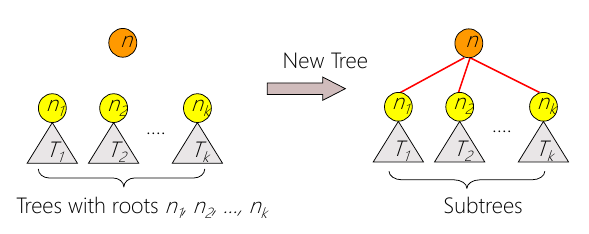
\includegraphics[]{img/treerecursivedef.png}
\end{center}

Some keywords : Parent/child, Ancestor/descendant, Siblings, Leaf, Depth, Height, Level.

\bigskip\noindent
\textbf{Binary Tree} : Every node has at most two children, Each child is designated as left child or a right child. (left child and right child are distict.)

\noindent
\textbf{Proper Tree} : Every node has 0 or 2 children.

\noindent
\textbf{Full Tree} : If it has a maximum number of nodes at each level. A full binary tree of height h has $2^{h+1} - 1$ nodes.
\bigskip

Node numbering :
\begin{enumerate}
    \item Zero-based numbering: \\
    \begin{tabular}{|c|c|c|c|c|c|c|c|c|c|}
        \hline
        \textbf{Array} & 0 & 1 & 2 & 3 & 4 & 5 & 6 & 7 & ... \\
        \hline
    \end{tabular}
    
    \bigskip\noindent
    Node 0 is the root, and the left child of node i is 2i+1, and the right child of node i is 2i+2. Parent node is $\lfloor \frac{i-1}{2} \rfloor$.
    \item One-based numbering: \\
    \begin{tabular}{|c|c|c|c|c|c|c|c|c|c|}
        \hline
        \textbf{Array} & 1 & 2 & 3 & 4 & 5 & 6 & 7 & 8 & ... \\
        \hline
    \end{tabular}

    \bigskip\noindent
    Node 1 is the root, and the left child of node i is 2i, and the right child of node i is 2i+1. Parent node is $\lfloor \frac{i}{2} \rfloor$.
\end{enumerate}

\noindent\textbf{Complete Binary Tree} : Relaxed definition of a full binary tree. A binary tree of height h is complete, if all levels possibly except h are completely full, and level h is filled from left to right.

\bigskip\noindent
\textbf{implementation}
\begin{itemize}
    \item Array implementation : Node numbered k is stored in an array tree[k].
    \item Linked Implementation : Struct Node {value, left, right}
\end{itemize}

\subsubsection*{Tree Traversal}

Tree traversal is passing through the tree and visiting each node exactly once (linearization). There are three ways to traverse the tree. (preorder, inorder, postorder). All of tree traversal is variant of depth-first search(DFS) complemented by  or recursive function call. Exceptionally, level-order traversal is breadth-first search(BFS) complemented by queue.
\begin{itemize}
    \item Preorder(T) = \textless n, Preorder($T_1$), Preorder($T_2$), ..., Preorder($T_k$)\textgreater
    \item Inorder(T) = \textless Inorder($T_1$), n, Inorder($T_2$), ..., Inorder($T_k$)\textgreater
    \item Postorder(T) = \textless Postorder($T_1$), Postorder($T_2$), ..., Postorder($T_k$), n\textgreater
\end{itemize}

\noindent Two type of traversal :
\begin{itemize}
    \item Depth-first traversal \\
    Go down first, recursive way, 3 variation : preorder, inorder, postorder
    \item Breadth-first traversal \\
    Go across first in same level, No variation, just level-order traversal
\end{itemize}

\noindent
For getting Unique binary tree by two traversals, only 3 types are valid : \textbf{(postorder and inorder), (preorder and inorder), (levelorder and inorder)}. 
Inorder are necessary to find left and right child, and postorder/preorder/levelorder are necessary to find root.

\bigskip
Some type of general tree implementations. This is example. 
\medskip
\textbf{Simple Approach} \\
\textbf{List-of-Children Approach} \\
\textbf{Left-Child/Right-Sibling Approach} \\
\textbf{TODO}
% //TODO ---



\subsubsection*{Converting into a Binary Tree : Donald Knuth}
Input : general trees. Then leftmost child is left child, and right sibling is right child. Finally, remove the other links. It seems like rotating the tree clockwise by 45$\deg$. When going from parent to leftchild, level be increase by 1 from original tree, and when going from parent to rightchild, level be same as original tree. Preorder is same, Postorder of original will be Inorder of new binary tree.


\bigskip
\end{section}
\begin{section}
    {Priority Queue \& Heap}
\section*{Priority Queue}

\subsection*{Definition}

Priority queue consists of a set of elements (organized by priority, also called key).

For implement priority queue, there are obvious ways.
\begin{center}
    \begin{tabular}{p{5cm}cc}
        \hline
        & Insert & DeleteMin \\
        \hline
        Normal queue & $O(1)$ & $O(n)$ \\
        Unsorted linked list & $O(1)$ & $O(n)$ \\
        Sorted linked list & $O(n)$ & $O(1)$ \\
        \hline
    \end{tabular}
\end{center}

$O(n)$ seems to much... so we need to find a better way -> Heap!

\subsection*{Heap}

\textbf{heap property}
\begin{itemize}
    \item if B is a child node of A, then $p(A) \le p(B)$.
    \item Implies that an element with the lowest priority is always in the root node (mean-heap) $\leftrightarrow$ (max-heap)
\end{itemize}

To efficiently implenet to priority queue -> Insert and DeleteMin : $O(\log n)$

There are some types of heap : binary, binomial, fibonacci, 2-3, etc.

\subsubsection*{Binary Heap}

Binary Heap satisfying two properties.
(1) Complete binary tree (structural property) (can be implemented in an array), (2) Min tree (Heap order property) (p(node) $\le$ p(children))
\small{We call Complete Binary Tree as CBT.}

\begin{center}
    \includegraphics*[]{img/Meanheap.png}
\end{center}

\begin{itemize}
    \item Insert
    \item DeleteMin
\end{itemize}

\textbf{Change Min Heap to Max Heap}
% // TODO ---

\bigskip
\end{section}
\begin{section}
    {Sorting}

    \textbf{WOw! THIS already exists in SUMMARY! Note that.}\\
    In this part, It will show how elements can be sorted by each methods simply.
    \begin{itemize}
        \item Bubble Sort
        \item Selection Sort
        \item Insertion Sort
        \item Bucket Sort
        \item Merge Sort
        \item Quick Sort
        \item Heap Sort...?
    \end{itemize}

\bigskip
\end{section}
\begin{section}
    {Binary Search Tree}

\subsection*{Definition}
\begin{itemize}
    \item Insert
    \item Delete
    \item Search
\end{itemize}

\noindent\bigskip
\textbf{}

\end{section}
\begin{section}
    {AVL Tree}

Why use AVL tree?

Balance factor

Rotatie

\begin{itemize}
    \item Insert
    \begin{itemize}
        \item Unbalance - LL
        \item Unbalance - RR
        \item Unbalance - LR
        \item Unbalance - RL
    \end{itemize}
    \item Delete
    \item Search
\end{itemize}


\end{section}

\begin{center}
    \par\noindent\line(1, 0){500}
\end{center}

\textbf{TIP!}

\begin{itemize}
    \item Mergesort, quicksort are slower than Insertion sort when approximately $ n \le 15$
    \item When running quicksort, the ideal case is choosing the median key value.
    \begin{itemize}
        \item Use the first or last element, then if the input is sorted, it will be poor.
        \item Pick an element at random, but using a random number generator is expensive.
        \item So, we have to select the middle element.
        \item Using \textbf{median-of-three} rule : choose the median of the first, middle, and last element.
    \end{itemize}
    \item Comparing Quicksort vs Heapsort : Quicksort is faster than heap, however quicksort should never be used in application which require a guarantee of response time unless it is treated as an $O(n\log n)$ algorithm.
    \item Comparing Quicksort vs Mergesort : Quicksort can be implemented in-place, but mergesort can't. No additional memory is required as in Merge sort. In many cases, quicksort can avoid $O(n^2)$ by choosing a right pivot.
\end{itemize}


\bigskip
\textbf{Stable Sort} : insertion, bubble,merge, couting, bucket

\textbf{Unstable Sort} : quick, heap, shell, selection

\medskip
\textbf{Comparison sort} : bubble, selection, insertion, heap, merge, quick

\textbf{non-comparison sort} : counting, bucket, radix



\newpage

\begin{section}
    {Summary}
\end{section}

{\textbf{Datastructure}}

\medskip
\begin{center}
    \begin{tabular}{|c|c|c|c|p{5.5cm}|}
    \hline
    \textbf{Datastructure} & \textbf{Insert} & \textbf{Delete} & \textbf{Locate} & \textbf{Description} \\
    \hline\hline
    \textbf{Array-based list} & $O(n)$ & $O(n)$ & $O(n)$ & If you know the proper pointer when insert, then $O(1)$\\ \hline
    \textbf{Pointer-based list} & $O(1)$ & $O(1)$ & $O(n)$ & \\ \hline
    \textbf{Cursor-based list} & $O(1)$ & $O(1)$ & $O(1)$ &  \\ \hline
    \textbf{Array-Based Queue} & $O(1)$ & $O(1)$ & $O(n)$ &  \\ \hline
    \textbf{Linked Queue} & $O(1)$ & $O(1)$ & $O(n)$ & \\ \hline
    \textbf{Tree} & $O(n)$ & $O(n)$ & $O(n)$ & According to implementation types, it can be changed. Check some approach of trees. \\ \hline
    \textbf{Priority Queue} & $O(log n)$ & $O(log n)$ & $O(n)$ &  \\ \hline
    \textbf{Heaps} & $O(log n)$ & $O(log n)$ & $O(n)$ & \\ \hline
    \textbf{Binary Search Tree} & $O(log n)$ & $O(log n)$ & $O(log n)$ & worst case, $O(n)$ \\ \hline
    \textbf{AVL tree} & $O(log n)$ & $O(log n)$ & $O(log n)$ &  \\ \hline
    \end{tabular}
\end{center}
\medskip

{\textbf{Algorithm}}

\medskip
\begin{center}
    \begin{tabular}{|c|c|c|c|l|}
        \hline
        \textbf{Algorithm} & \textbf{Worst} & \textbf{Average} & \textbf{Best} & \textbf{Description} \\
        \hline\hline
        \textbf{Bubble sort} & $O(n^2)$ & $\Theta (n^2)$ & $\Omega (n)$ & Comparison, Stable Sort\\ \hline
        \textbf{Insertion sort} & $O(n^2)$ & $\Theta (n^2)$ & $\Omega (n)$ & Comparison, Stable Sort\\ \hline
        \textbf{Selection sort} & $O(n^2)$ & $\Theta (n^2)$ & $\Omega (n^2)$ & Comparison, Unstable Sort\\ \hline
        \textbf{Bucket sort} & $O(n^2)$ & $\Theta (n+N)$ & $\Omega (n+N)$ &
        \begin{tabular}{@{}l@{}}
            Non-Comparison, Stable Sort. \\
            $N$ is the number of buckets. \\
            Worst is that all is in only one.
        \end{tabular} \\ \hline
        \textbf{Merge sort} & $O(n\log n)$ & $\Theta (n\log n)$ & $\Omega (n\log n)$ &
        \begin{tabular}{@{}l@{}}
            Comparison, Stable Sort, \\
            Divide-and-Conquer \\
            Recursive(up\&down) \\
            -or, Non-recursive(upward)
        \end{tabular} \\ \hline
        \textbf{Quicksort} & $O(n^2)$ & $\Theta (n\log n)$ & $\Omega (n\log n)$ &
        \begin{tabular}{@{}l@{}}
            Comparison, Unstable Sort, \\
            Worst is that pivot selection \\
            -is not balanced.
        \end{tabular} \\ \hline
        \textbf{Heap sort} & $O(n\log n)$ & $\Theta (n\log n)$ & $\Omega (n\log n)$ & Comparison, Unstable Sort \\ \hline
    \end{tabular}
\end{center}

\bigskip


\end{document}